%\IfFileExists{revtex4-1.cls}{\documentclass[prd, twocolumn, lengthcheck, superscriptaddress, showpacs, letterpaper, footinbib]{revtex4-1}}{ 
%\IfFileExists{revtex4.cls}{\documentclass[prd, twocolumn, lengthcheck, superscriptaddress, showpacs, letterpaper]{revtex4}}{}}
\documentclass{emulateapj}

%\documentclass[prd, twocolumn, lengthcheck,superscriptaddress, showpacs, letterpaper, footinbib]{revtex4}
%\documentclass[lengthcheck,superscriptaddress,showpacs,letterpaper,nofootinbib]{article}
\usepackage{ifpdf}
\usepackage[bookmarks=false]{hyperref}
\pdfoutput=1
\usepackage[usenames,dvipsnames]{color}
\usepackage{graphicx}
\usepackage{graphics}  
  \usepackage{float}
%\restylefloat{table}
\usepackage{amsmath}
\usepackage{amssymb}
\usepackage{acronym}
\usepackage{multirow}
\usepackage{xspace}
%\restylefloat{figure}
\usepackage{units}
\usepackage{dcolumn}
\usepackage{ulem}

\def\aj{Astron. J.}                 % Astronomical Journal
\def\apj{Astrophys. J.}                % Astrophysical Journal
\def\apjl{Astrophys. J. Lett.}             % Astrophysical Journal, Letters
\def\pasj{PASJ}
\def\apjs{Astrophys. J., Suppl. Ser.}              % Astrophysical Journal, Supplement
\def\mnras{Mon. Not. R. Astron. Soc.}            % Monthly Notices of the RAS
\def\prd{Phys. Rev. D}       % Physical Review D
\def\prl{Phys. Rev. Lett.}    % Physical Review Letters
\def\cqg{Class. Quant. Grav.}%Classical and Quantum Gravity
\def\araa{Annu. Rev. Astron. Astrophys.}             % Annual Review of Astron and Astrophys
\def\nat{Nature}              % Nature
\def\aap{Astron. Astrophys.}                % Astronomy and
                                % Astrophysics
\def\jasa{J. Am. Stat. Assoc.}
\def\pccp{Phys. Chem. Chem. Phys.}
\def\jrssb{J. R. Stat. Soc. B}
\def\aipcs{AIP Conf. Ser.}
\def\jcp{J. Chem. Phys.}

\newcommand{\carl}[1]{{\color{red}  #1}}
\newcommand{\ilya}[1]{{\color{blue} #1}}
\newcommand{\ben}[1]{{\color{green} #1}}
\newcommand{\will}[1]{{\color{cyan} #1}}


\begin{document}
\title{Basic Parameter estimation of Binary Neutron Star Systems by the Advanced LIGO/VIRGO Network}
\author{Carl L. Rodriguez}
\email{carlrodriguez2015@u.northwestern.edu}
\affiliation{Center for Interdisciplinary Exploration and Research in Astrophysics (CIERA) \& Dept.~of Physics and Astronomy, Northwestern University, 2145 Sheridan Rd, Evanston, IL 60208, USA}

\begin{abstract}
\end{abstract}

\maketitle
\section{Introduction}

 By 2016 (\carl{?}), the field of gravitational-wave astrophysics will mature from a speculative scientific genre into an ideal tool for exploring the gravitational side of the universe.
 Within the next few years, the first generation of gravitational-wave detectors capable of regularly resolving astrophysical sources will come online \carl{cite}.   The Advanced LIGO and VIRGO detectors will provide  the first insights into the final moment of binary compact object mergers, including the merger of binary neutron star systems.  Intense preparations are currently underway to prepare to characterize and extract as much physical information as possible from these signals.
 
The mergers of binary neutron stars are expected to be the most ubiquitous source in the advanced detector era \carl{cite}.   Models from stellar evolution suggest that the number of binary neutron star mergers within Advanced LIGO/VIRGO's detection horizon could reach into the hundreds per year \carl{cite}.  Although the peak sensitivity of ground-based detectors is not focused on the frequency at which BNS systems merge, it should still be possible to extract information about both strong field gravitational physics \carl{cite} and the hydrodynamics of dense matter (e.g. the equation of state of nuclear matter) \carl{cite}.  As such, BNS systems will likely form the ``bread and butter'' of the compact object efforts in the coming years \carl{the high-mass folks might not like this, but fuck 'em}.

Of course, in this context, one must distinguish between the detection of such events, and the precision measurement of the relevant physical parameters.   There are two separate issues to consider in this context: the detection of BNS systems will be performed with a matched filtering approach, which allows one to search the time domain data at a sufficiently fast rate \carl{[yeah that phrasing sucks]} by comparing the data stream to a bank of theoretical templates.  When the overlap between one of the template waveforms and the detector output is sufficiently large (97\%), a detection is claimed.  However, the parameter space of our signals can be highly degenerate, with several locations in parameter space corresponding to near identical waveforms.  In order to fully realize the science potential of these instruments, we must perform a full exploration of the parameter space for each detection.  By analyzing each candidate's parameter space with fully Bayesian techniques and proper sampling, we will be able to make precise, scientifically meaningful statements about the composition and formation of these objections.  To this end, we employ a Markov-Chain Monte Carlo sampling algorithm, included in the LIGO Application Library parameter estimation code, \texttt{LALInferenceMCMC}.  

By employing the full parameter estimation machinery that will eventually be used in the Advanced Detector era, our results give the first estimate at the realistic capabilities of Advanced ground-based detectors.  Until recently, the majority of studies have employed the Fisher matrix formalism as it was first adapted for gravitational-wave parameter estimation by \cite{FinnDetection}.  While each of these studies (\cite{PoissonWill,CutlerFlanagan,ArunPE}, among many others) have done their due diligence in pointing out the limitations and flaws of the Fisher Information Matrix, there has been no study which states the BNS parameter estimation capabilities of Advanced LIGO/VIRGO via the techniques that will eventually be employed.  The recent work of \cite{Vallisneri} and our own work \citep{Inadequacies} has demonstrated that the Fisher matrix cannot even be treated as a lower bound on the standard deviations about certain parameters (particularly the masses) measurable in advanced detectors.

In this paper, we perform a systematic study of the statistical uncertainty with which the Advanced LIGO network will be able to measure the basic parameters of binary neutron stars.  In section \ref{BNSsection}, we review some of the basic physics of gravitational waves from binary neutron stars, including the potential science case to be made with Advanced LIGO.  In section \ref{PEsection}, we describe the machinery of our parameter estimation code, \texttt{LALInferenceMCMC}, as well as the gravitational-wave template used for signal extraction.   In section \ref{ResultsSection}, we 

 
\begin{itemize}
 \item BNS source
\item PE vs detection
\item Why not FIM
\item Overview
\end{itemize}

\section{BNS systems}
\label{BNSsection}
\begin{itemize}
\item expected rates
\item interesting physics
\item Expected parameters (non spinning, SNR distribution, etc)
\item waveform issues
\end{itemize}

\section{Parameter Estimation}
\label{PEsection}

\begin{itemize}
\item parameter estimation setup
\item MCMC
\item Waveform model
\end{itemize}
\label{peSection}

We begin by introducing a Bayesian formalism for parameter estimation. 
%Before offering a brief derivation of the FIM, a few preliminary
%techniques must be introduced.  First,
We assume that the time-domain signal in our gravitational wave
network can be written as a combination of a gravitational
waveform $h_0$ and the noise of the detector $n$.  We further assume
that this noise is stationary and Gaussian with mean zero.  Therefore,
the detector output is simply
\begin{equation}
s = n + h_0 .
\label{SignalAddition}
\end{equation}
Since our noise is assumed to be Gaussian, we can write the
probability of a specific signal realization $s$ as the probability
that our signal is Gaussian once the waveform has been subtracted
\begin{align}
  p(s | \boldsymbol{\theta}) &\propto \exp\left[-\frac{1}{2}\left<n|n
    \right>\right] \nonumber \\ &= \exp\left[-\frac{1}{2}\left < s -
    h(\boldsymbol{\theta}) | s-h(\boldsymbol{\theta})\right >\right] ,
  \label{likelihood}
\end{align}
where $\boldsymbol{\theta}$ is the set of parameters for our template
waveforms.The inner product, $\left< ~|~ \right> $, is defined using the noise
spectrum of the detectors as
\begin{equation}
  \left<a|b\right> \equiv 4 \Re \int \frac{\tilde{a}(f)\tilde{b}^*(f)}{S_n(f)} df ,
  \label{innerProduct}
\end{equation}
where $S_n(f)$ is the one-sided power spectral density as a function
of frequency, and $\tilde{a}(f)$ and $\tilde{b}(f)$ are the Fourier
transforms of the time-domain signals $a(t)$ and $b(t)$.
 
Once we have the likelihood of the signal \eqref{likelihood}, we
employ Bayes Rule to obtain the posterior probability of the system
parameters $\boldsymbol{\theta}$ given the signal $s$ as
\begin{align}
  p(\boldsymbol{\theta} | s) &= \frac{p(\boldsymbol{\theta})p(s | \boldsymbol{\theta})}{p(s)} \nonumber\\
  & \propto p(\boldsymbol{\theta}) \exp\left[-\frac{1}{2}\big < s - h(\boldsymbol{\theta}) | s-h(\boldsymbol{\theta}) \big > \right] ,
  \label{posterior}
\end{align}
where $p(\boldsymbol{\theta})$ are the prior probabilities on our
source parameters and $p(s)$ is a normalization constant.  Our prior
information can come from physics limits in the parameter space, or
from our \textit{a priori} knowledge of astrophysical systems. If we
pick a set of parameters $\boldsymbol{\theta}$ such that
$h(\boldsymbol{\theta}) = h_0$, then our posterior \eqref{posterior}
will be near a global maximum; however, the presence of noise will in
general deflect the maximum of our posterior away from the value at
$\boldsymbol{\theta}_0$. That is, in the presence of noise, there is
no guarantee that the maximum-likelihood of our signal corresponds to
the true parameters of the system.  Hence our use of the term
``best-fit parameters'' (\citep{CutlerFlanagan}), particularly when
discussing the point in parameter space where the FIM is evaluated.
The goal of parameter estimation is to sample the available parameter
space, considering all areas of posterior support, to determine best
estimates on the parameters of the signal and their uncertainties.  We
will discuss one such sampling technique, Markov-Chain Monte Carlo, in
\ref{MCMCSection}.

  
\subsection{Parameter estimation via Markov-Chain Monte Carlo}
\label{MCMCSection}
  
Our parameter estimation code, \texttt{LALInferenceMCMC}, is an
enhancement of the previously described MCMC parameter estimation code
\texttt{SpinSpiral} \citep{spinspiral2009, spinspiral2010}.  The basic
description of the Markov-Chain Monte Carlo via the
Metropolis-Hastings algorithm is as follows \citep{Gilks99}:
  
\begin{enumerate}
\item Pick an initial point in the parameter space
  ($\boldsymbol{\theta_{\text{old}}}$), and then propose a random
  ``jump'' to a new set of waveform parameters,
  $\boldsymbol{\theta_{\text{new}}}$.  The jump follows the
  (conditional) probability distribution $q\left(
  \boldsymbol{\theta_{\text{new}}} | \boldsymbol{\theta_{\text{old}}}
  \right)$.
\item Calculate the posterior probability,
  $p(\boldsymbol{\theta_{\text{new}}}|s)$, of the new parameters using
  \eqref{likelihood} and \eqref{posterior}.
\item Accept the new parameters with probability 
  \begin{equation}
    p_\mathrm{accept} = \min \left[ 1, \frac{p(\boldsymbol{\theta_{\text{new}}}|s) q\left(\boldsymbol{\theta_{\text{old}}} | \boldsymbol{\theta_{\text{new}}} \right)}{p(\boldsymbol{\theta_{\text{old}}}|s) q\left(\boldsymbol{\theta_{\text{new}}} | \boldsymbol{\theta_{\text{old}}} \right)} \right].
  \end{equation}
  If the new parameters are accepted, record
  $\boldsymbol{\theta_\text{new}}$ and repeat with
  $\boldsymbol{\theta_\text{old}} \gets
  \boldsymbol{\theta_\text{new}}$; otherwise, record
  $\boldsymbol{\theta_\text{old}}$, and repeat.
\end{enumerate} 
  
The above procedure is designed to record a chain of samples whose
distribution is $p\left(\boldsymbol{\theta}|s\right)$.  Depending on
the proposal distribution, $q$, the convergence (mixing) of the chain
may be rapid or slow.  We employ multiple optimization techniques,
including both specially-crafted $q$ and parallel tempering, to ensure
adequate mixing of the Markov Chains throughout our parameter space.
The details of the algorithm can be found in
\citep{Sluys08,spinspiral2009, spinspiral2010}.
  
 
\subsection{Waveform Model}
\label{waveformSection}
  
We use a frequency domain waveform accurate up to $3.5$
post-Newtonian (pN) order in phase and amplitude.  We restrict ourselves to
quasi-circular waveforms as a simplifying assumption.  The standard
form of our waveform model, known as the \textit{TaylorF2}
approximant, is calculated via the stationary phase approximation \citep{BuonannoWaveform}.
  In this setup, the gravitational-wave
amplitude is given by
\begin{equation}
\tilde{h}(f) = A f^{-7/6}e^{i \psi(f)},
\label{amplitude}
\end{equation}
where $A \propto \mathcal{M}_c^{5/6}\Theta(\text{angle})/D$, $D$ is
the luminosity distance of the binary, and $\psi(f)$ is the pN phase.
$\Theta(\text{angle})$ is a function of the orbital orientation with
respect to the detector network in terms of the sky position, orbital
inclination, and the wave polarization.  In addition to the total
mass, $M\equiv m_1+m_2$, it is convenient to work with the
\textit{symmetric mass ratio} and \textit{chirp mass}, defined by
\begin{equation}
  \eta\equiv m_1m_2/M^2~~~~\text{and}~~~~\mathcal{M}_c = \eta^{3/5}M,
\end{equation}
respectively.  Then, in terms of the Newtonian orbital velocity
$v=(\pi M f)^{1/3}$, the 2pN phase is
\begin{equation}
\psi(f) = 2 \pi f t_c - \phi_0 + \frac{\pi}{4} + \frac{3}{128 \eta}v^{-5}\sum^{4}_{k=0}\alpha_{k}v^k
\label{phase}
\end{equation}
with coefficients
\begin{align}
\alpha_0 &= 1\\
\alpha_1 &= 0 \nonumber\\
\alpha_2 &= \frac{20}{9}\left(\frac{743}{336}+\frac{11}{4}\eta\right)\nonumber\\
\alpha_3 &= -16\pi \nonumber\\
\alpha_4 &= 10\left(\frac{3058673}{1016064}+\frac{5249}{1008}\eta+\frac{617}{144}\eta^2  \right) . \nonumber\\
\alpha_5 &= \pi\left(\frac{38645}{756}-\frac{65}{9}\eta\right)\left(1+3\log\left(\frac{v}{v_{\text{ISCO}}}\right)\right)\nonumber\\
\alpha_6 &= \frac{11583231236531}{4694215680} - \frac{640}{3}\pi^2 - \frac{6848}{21}\gamma_{\text{euler}} \nonumber\\
         &~~- \frac{6848}{21} \log\left(4 \frac{v}{v_{\text{ISCO}}}\right) -\left(\frac{15737765635}{3048192}-\frac{2255}{12}\pi^2\right)\eta\nonumber\\
           &~~+ \frac{76055}{1728}\eta^2 - \frac{127825}{1296}\eta^3\nonumber\\
\alpha_7 &= \pi\left(\frac{77096675}{254016}+\frac{1014115}{3024}\eta - \frac{36865}{368}\eta^2\right)\nonumber
\end{align}
The terms $t_c$ and $\phi_0$ in equation (\ref{phase}) are constants
of integration, referring to the chirp time and coalescence phase,
respectively.  Although uninteresting physically, they must be
accounted for in any parameter estimation study of the waveform phase.

To perform the integral defined in \eqref{innerProduct}, we used an
analytic noise curve for the Initial LIGO configuration, provided in
\citet{DarmourNoiseCurve}, which takes the form:
\begin{align}
 S_h(f)=&S_0\Big[ \left(\frac{4.49 f}{f_0} \right)^{-56} + \nonumber\\
 &\left(\frac{0.16f}{f_0}\right) ^{-4.52}+0.52+0.32\left( \frac{f}{f_0}\right) ^2\Big],
 \label{PSD}
\end{align}
where $f_0 = 150~\text{Hz}$, and $S_0 = 9\times
10^{-46}\text{Hz}^{-1}$.  We consider the complete initial detector
network consisting of the two LIGO sites (in Hanford, WA and
Livingston, LA) and the Virgo site (in Pisa), although for simplicity
we use the Initial LIGO sensitivity for all three detectors.  For a
multi-detector network, the noise-weighted inner products
\eqref{innerProduct} combine linearly, allowing us to use the above
formalism with minimal modification.  We integrate the inner product
from a lower frequency cutoff of $40\text{Hz}$ to the
innermost-stable-circular orbit of the system in question, which for a
non-spinning binary is given by
\begin{equation}
  \pi f_{\text{ISCO}} = \frac{1}{6^{3/2}M}.
  \label{ISCOFrequency}
\end{equation}
   
In addition to the intrinsic parameters listed above ($\mathcal{M}_c,
\eta, \phi_0,t_c$), we include an additional 5 extrinsic parameters in
our parameter estimation, in order to explore how a full parameter
estimation study on real data, including parameters such as sky
location, will compare to their FIM counterparts.  This leads to our
9-dimensional parameter space for non-spinning systems:
\begin{equation}
\boldsymbol{\theta} =  (\mathcal{M}_c, \eta, \phi_0,t_c,D,\iota,\psi,\alpha,\delta)
\label{parameterspace}
\end{equation}
where $D$ is the luminosity distance to the binary, $\iota$ is the
orbital inclination, $\psi$ the gravitational-wave polarization, and
$\alpha$ and $\delta$ the right ascension and declination of the
source on the sky.

Note that the signal-to-noise ratio (SNR) of a gravitational wave in a
single detector is
\begin{equation}
  \rho \equiv \frac{4}{\sigma} \int^{\infty}_{0}\frac{| \tilde{s}(f)\tilde{h}^{*}(f)|}{S_{n}(f)}df
  \label{formalSNR}
\end{equation}
where $\rho$ is the SNR and $\tilde s(f)$ and $\tilde{h}^{*}(f)$ are
the frequency-domain signal and template, respectively.  The SNRs for
multiple detectors add in quadrature.  The normalization $\sigma$ is
given by
\begin{equation}
  \sigma^2 = 4\int^{\infty}_{0}\frac{| \tilde{h}(f)|^2}{S_n(f)}df.
  \label{SNRnorm}
\end{equation}
For our MCMC analysis, we compute the SNR directly using
\eqref{formalSNR}.  In the case of the FIM, we approximate the SNR
using $\sigma$ from equation (\ref{SNRnorm}) for a network of
detectors as
\begin{equation}
\rho = \sqrt{\sum_i \sigma_i^2}
\label{snr}
\end{equation}
where the index $i$ refers to the signal and noise spectrum of the
$i^{\text{th}}$ detector.  It should be noted that equation
\eqref{snr} is only valid in case of stationary Gaussian noise.

\begin{figure*}[h]
\begin{center}
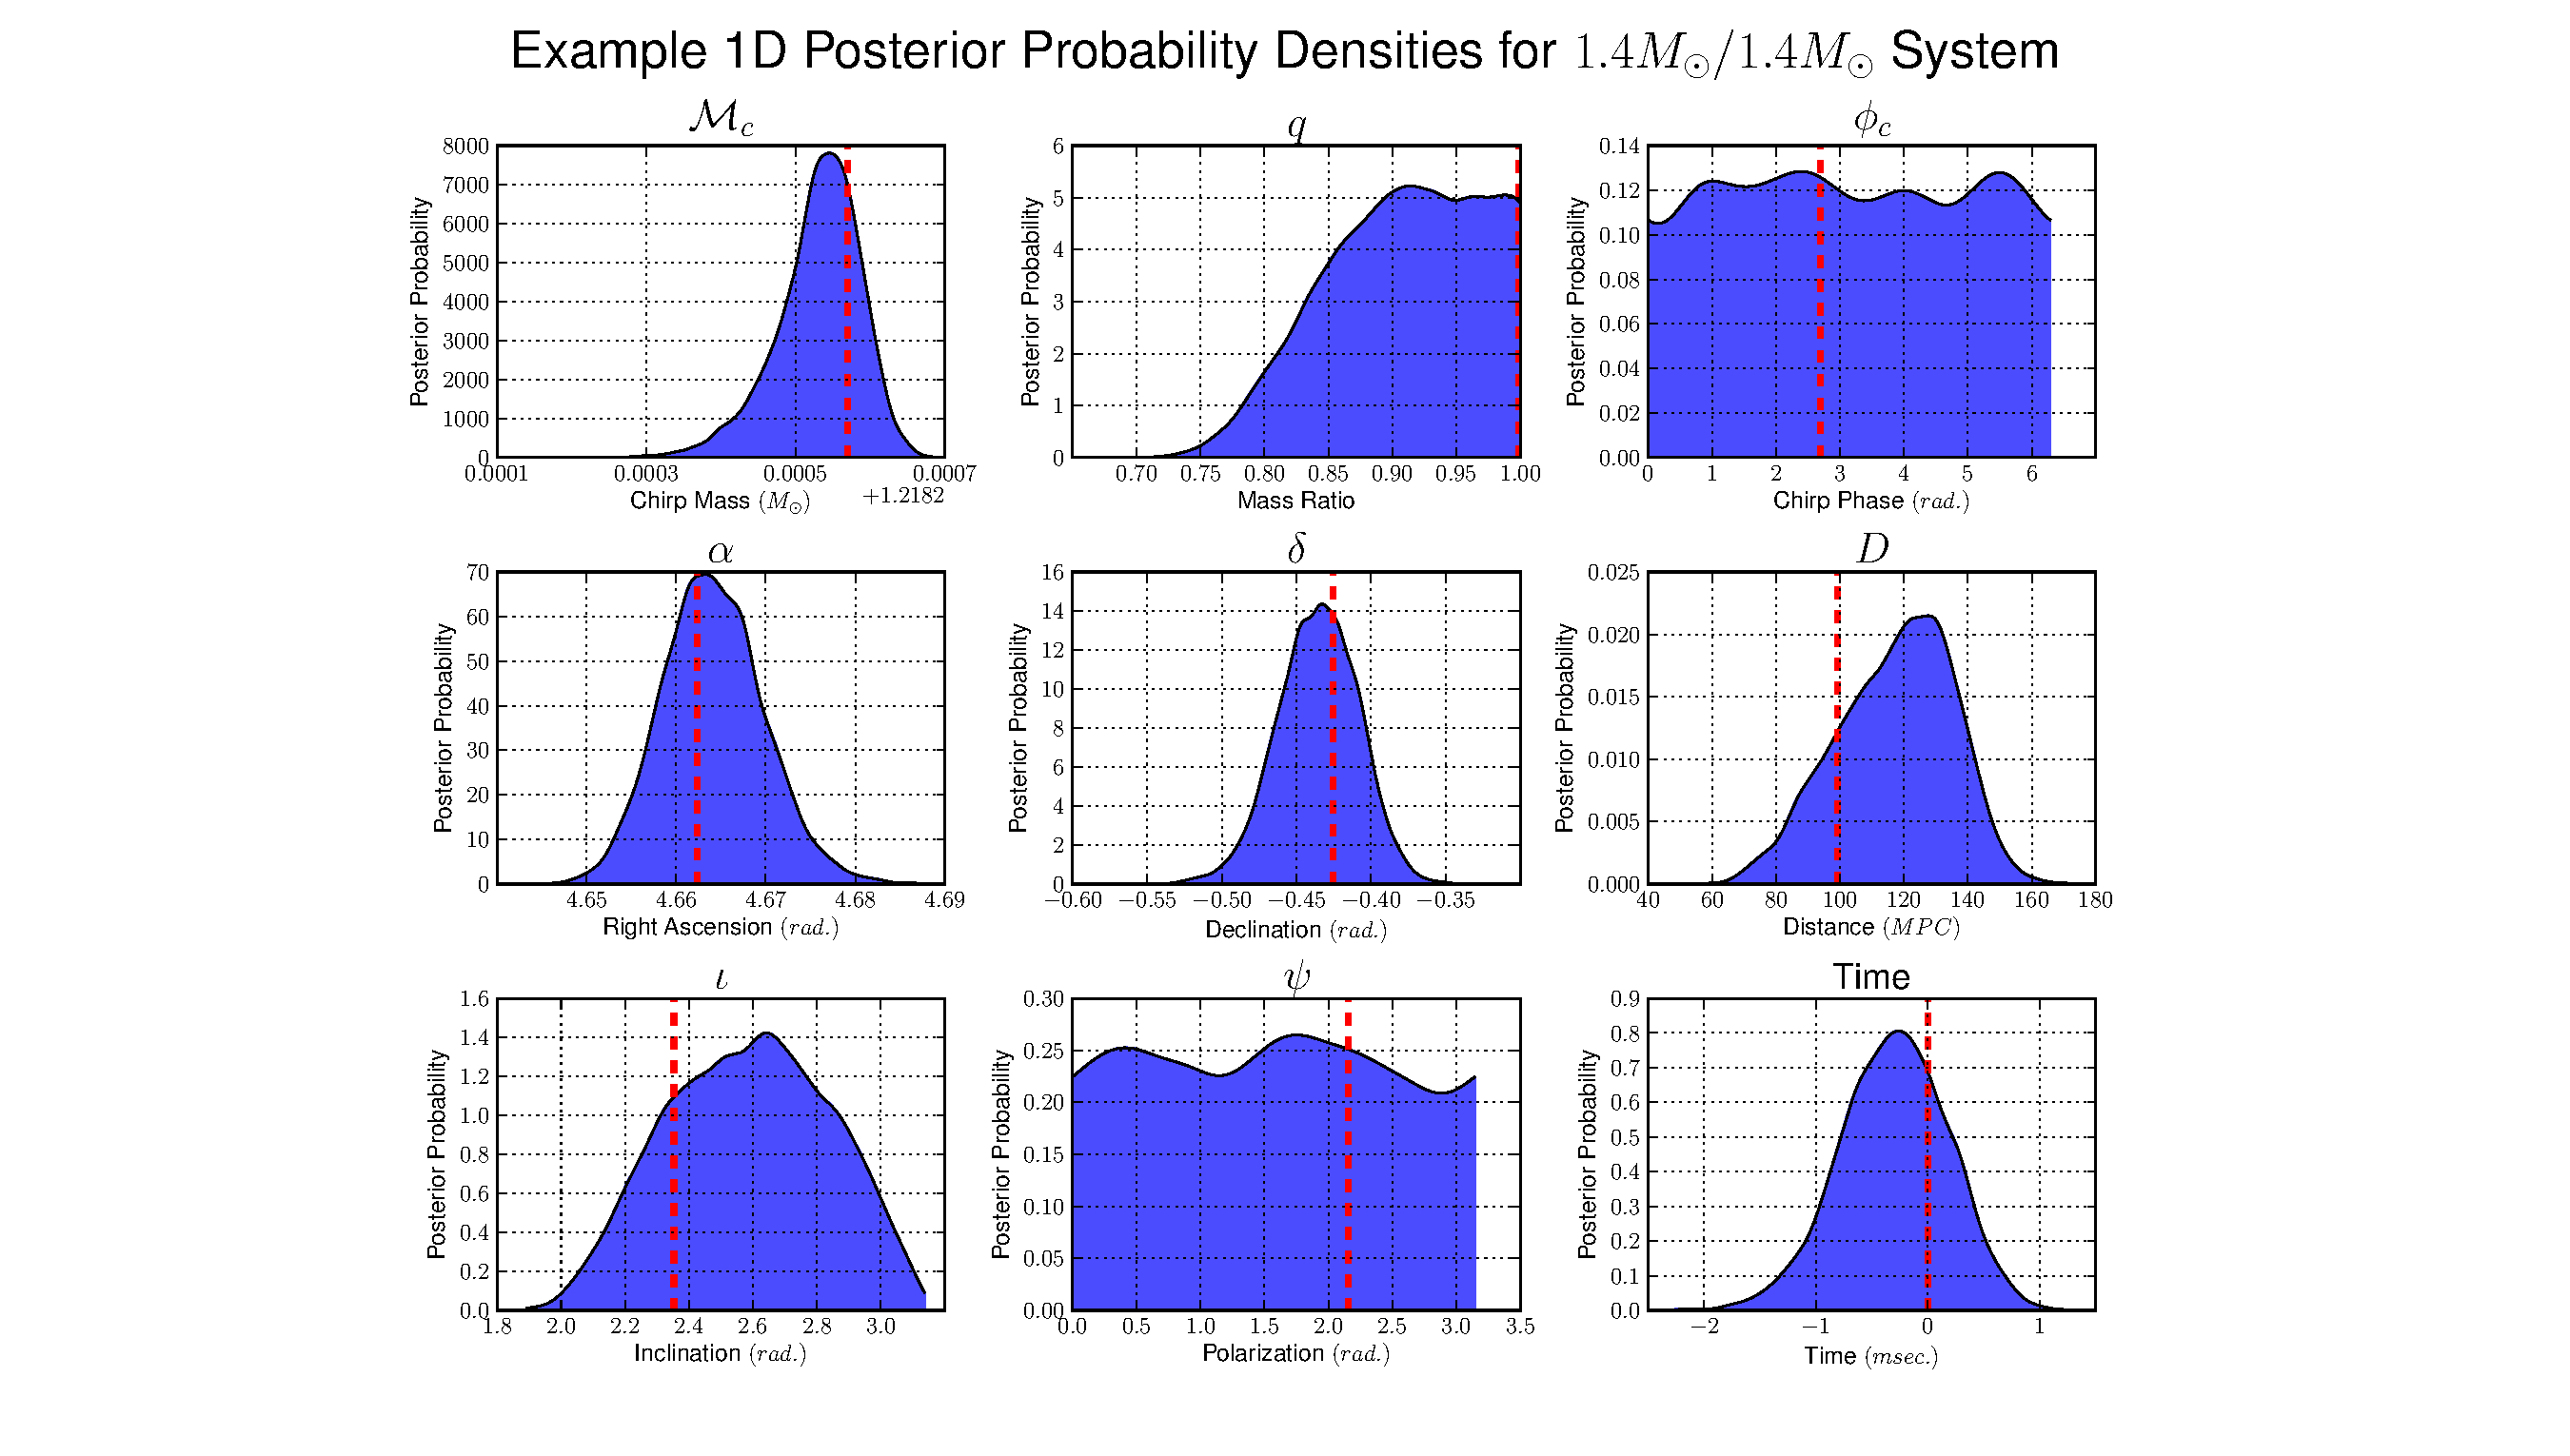
\includegraphics[trim=0cm 0cm 0cm 0cm, clip=true,scale=0.57]{9dpdf.pdf}
%\begin{array}{ccc} 
%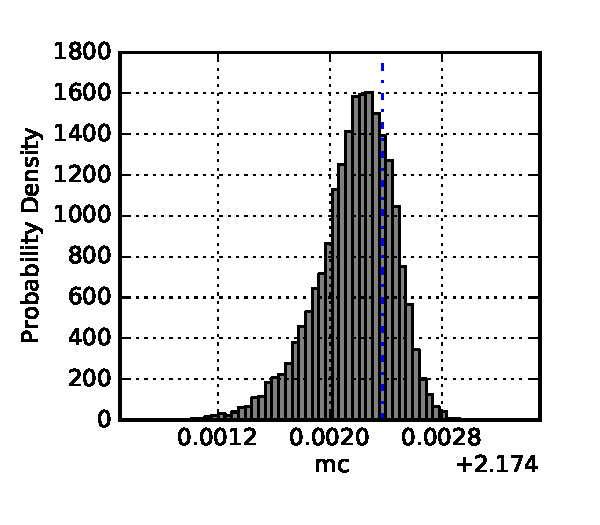
\includegraphics[width=2.2in]{1dpdfs/mc.pdf} &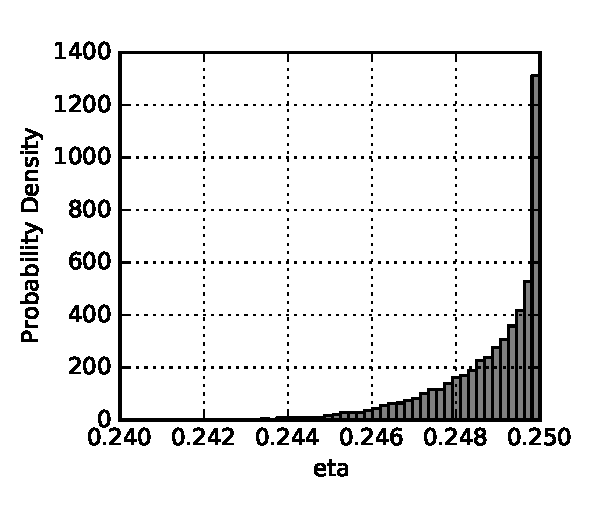
\includegraphics[width=2.2in]{1dpdfs/eta.pdf}  & 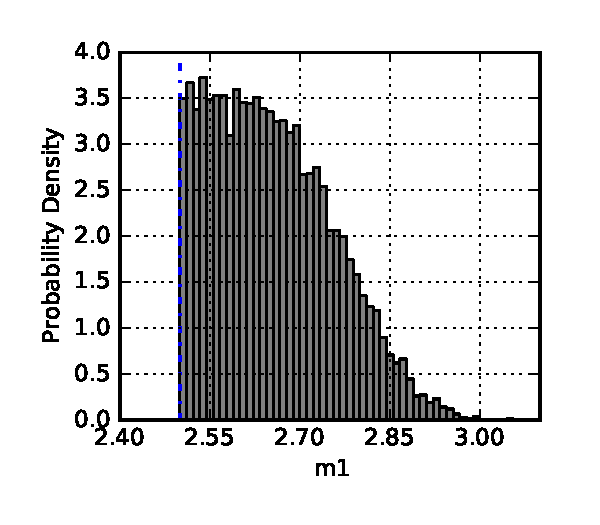
\includegraphics[width=2.2in]{1dpdfs/m1.pdf}\\
%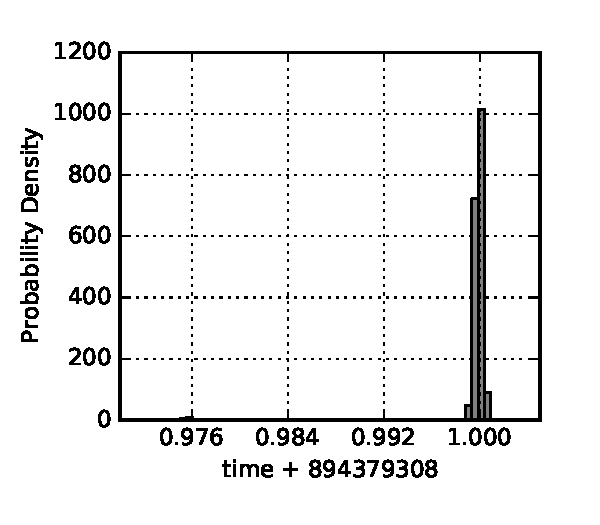
\includegraphics[width=2.2in]{1dpdfs/time.pdf} &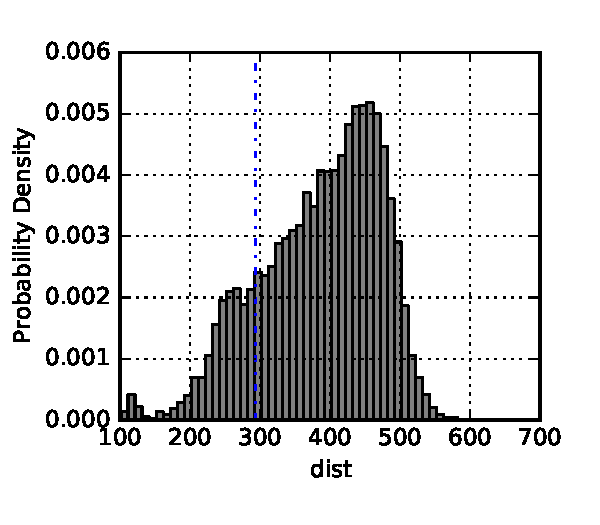
\includegraphics[width=2.2in]{1dpdfs/dist.pdf}  &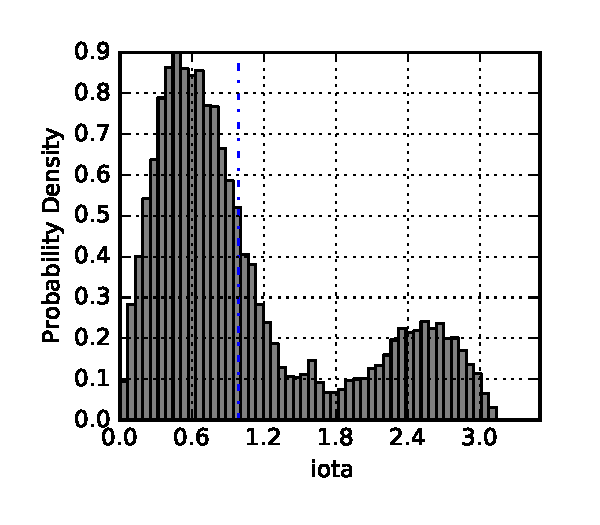
\includegraphics[width=2.2in]{1dpdfs/iota.pdf}\\
%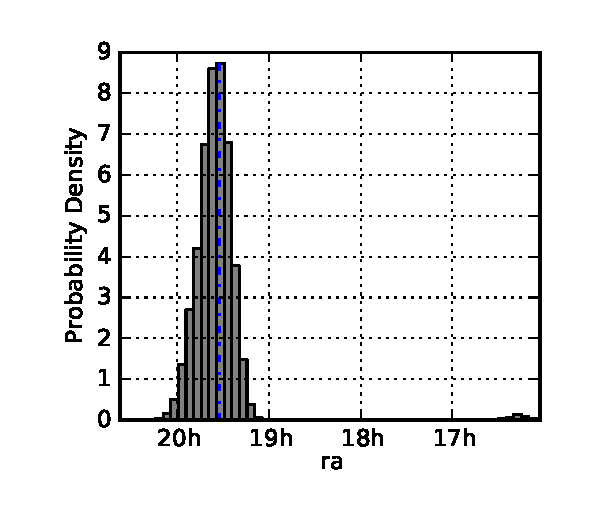
\includegraphics[width=2.2in]{1dpdfs/ra.pdf} & 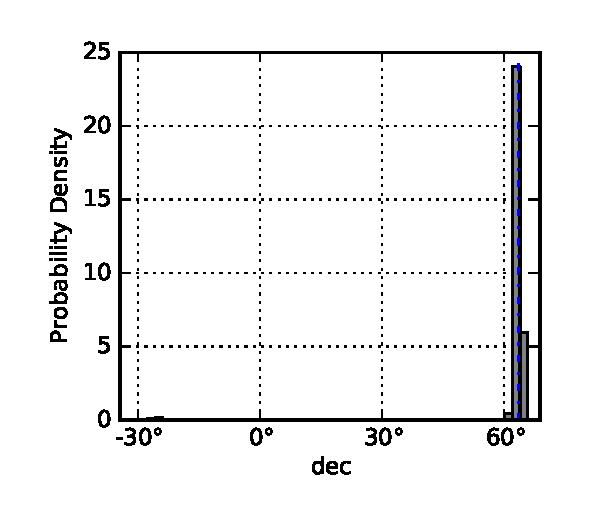
\includegraphics[width=2.2in]{1dpdfs/dec.pdf} & 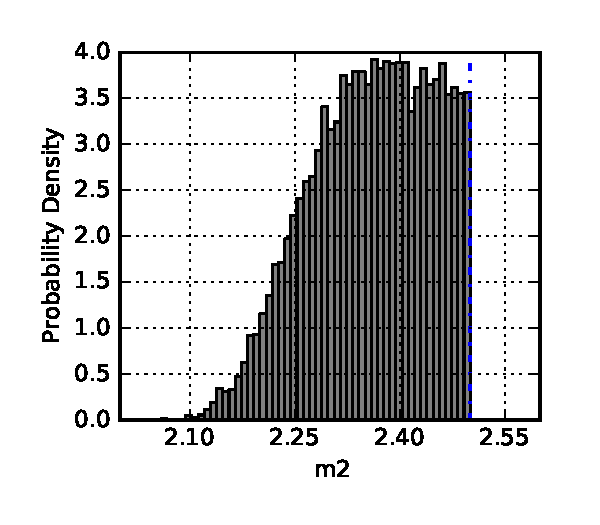
\includegraphics[width=2.2in]{1dpdfs/m2.pdf}
%\end{array}$
\end{center}
\caption{Marginalized 1D posterior probability density functions taken from a typical $1.4M_{\odot}/1.4M_{\odot}$ BNS system.  We have plotted each of the 9 parameters for our non-spinning BNS problem as stated in section \ref{waveformSection}.  Note how, even for parameters with excellent recovery, the peak of the 1D Gaussian is displaced from the injected value (in dashed red).  This is not due to a systematic bias, but is caused by the marginalization of a single dimmension from the full 9D posterior space.}
\end{figure*}


\begin{figure*}[h!]
  \centering
 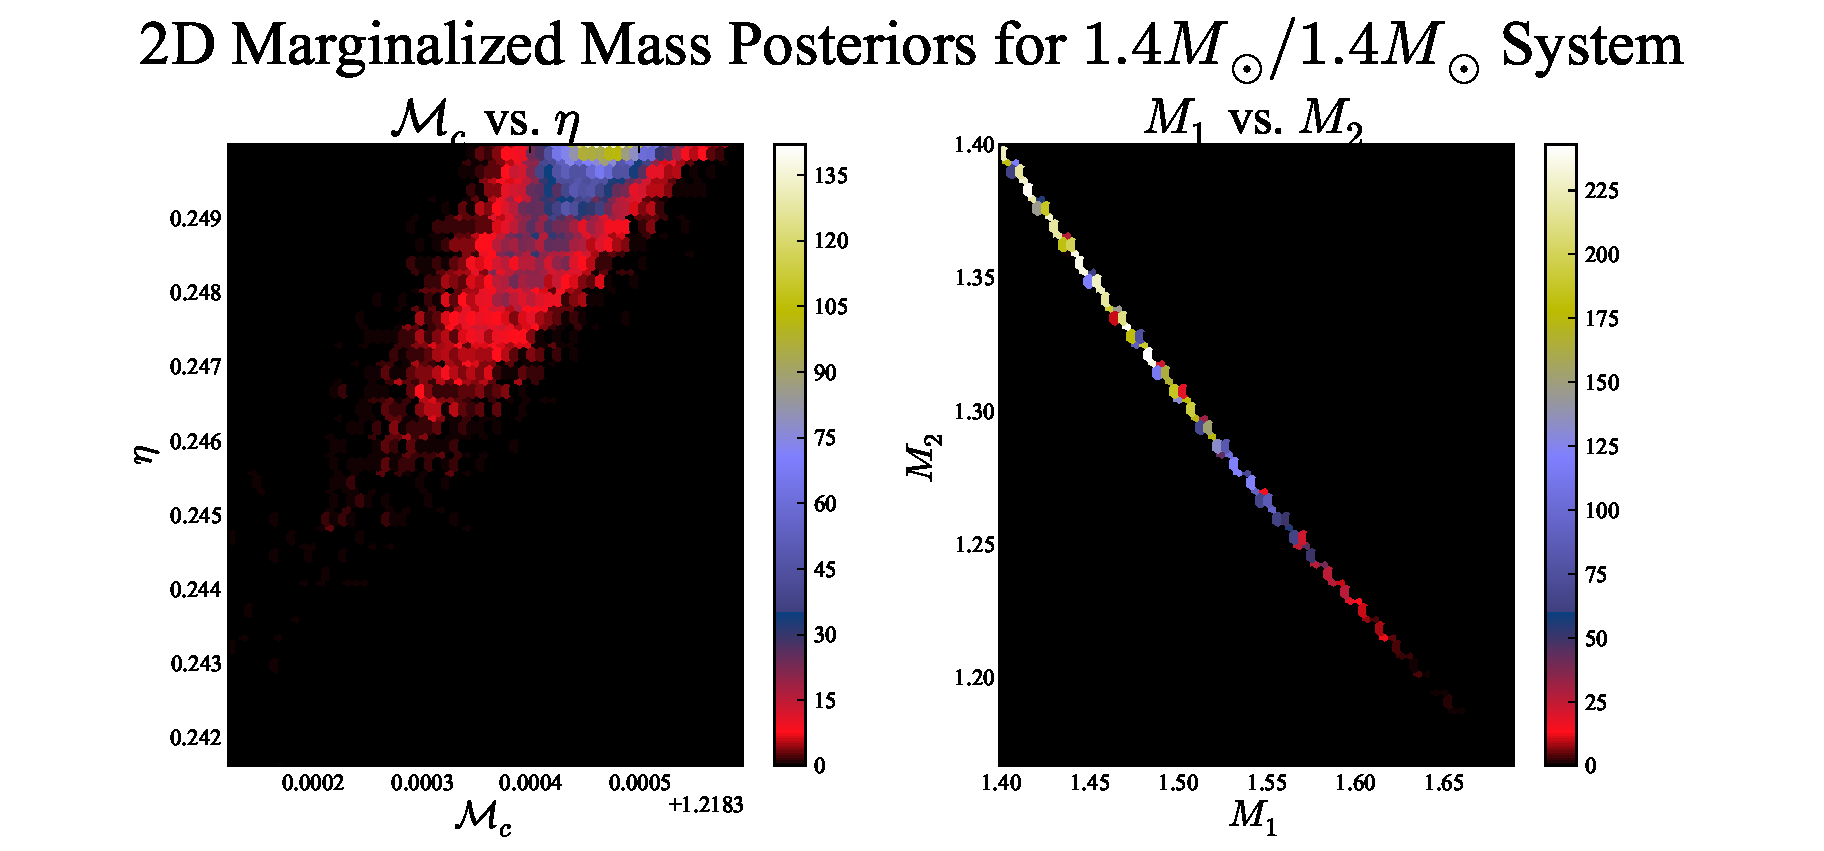
\includegraphics[trim=2cm 0cm 2cm 0cm, clip=true,scale=0.63]{1414masses2D.pdf}
 \label{1414masses}
 \caption{2D marginalized posterior probability density functions for the mass parameters recovered in typical a $1.4M_{\odot}/1.4M_{\odot}$ system.  The posteriors are plotted in terms of parameters used in the waveform, chirp mass ($\mathcal{M}_C$) and the reduced mass ratio ($\eta$), and in the individual component masses of the binary ($M_1$ and $M_2$).  In the $\mathcal{M}_c$-$\eta$ space, the posterior would resemble a Gaussian if not for the limitation of $\eta \leq 0.25$.  The presence of the $\eta$ cutoff and the convention that $M_1 \geq M_2$ inform the non-Gaussian features present.  When projected as 1D marginalized posteriors, the component masses resemble the posterior PDFs shown in figure \ref{masses}.}
\end{figure*}


\begin{figure*}[h!]
  \centering
 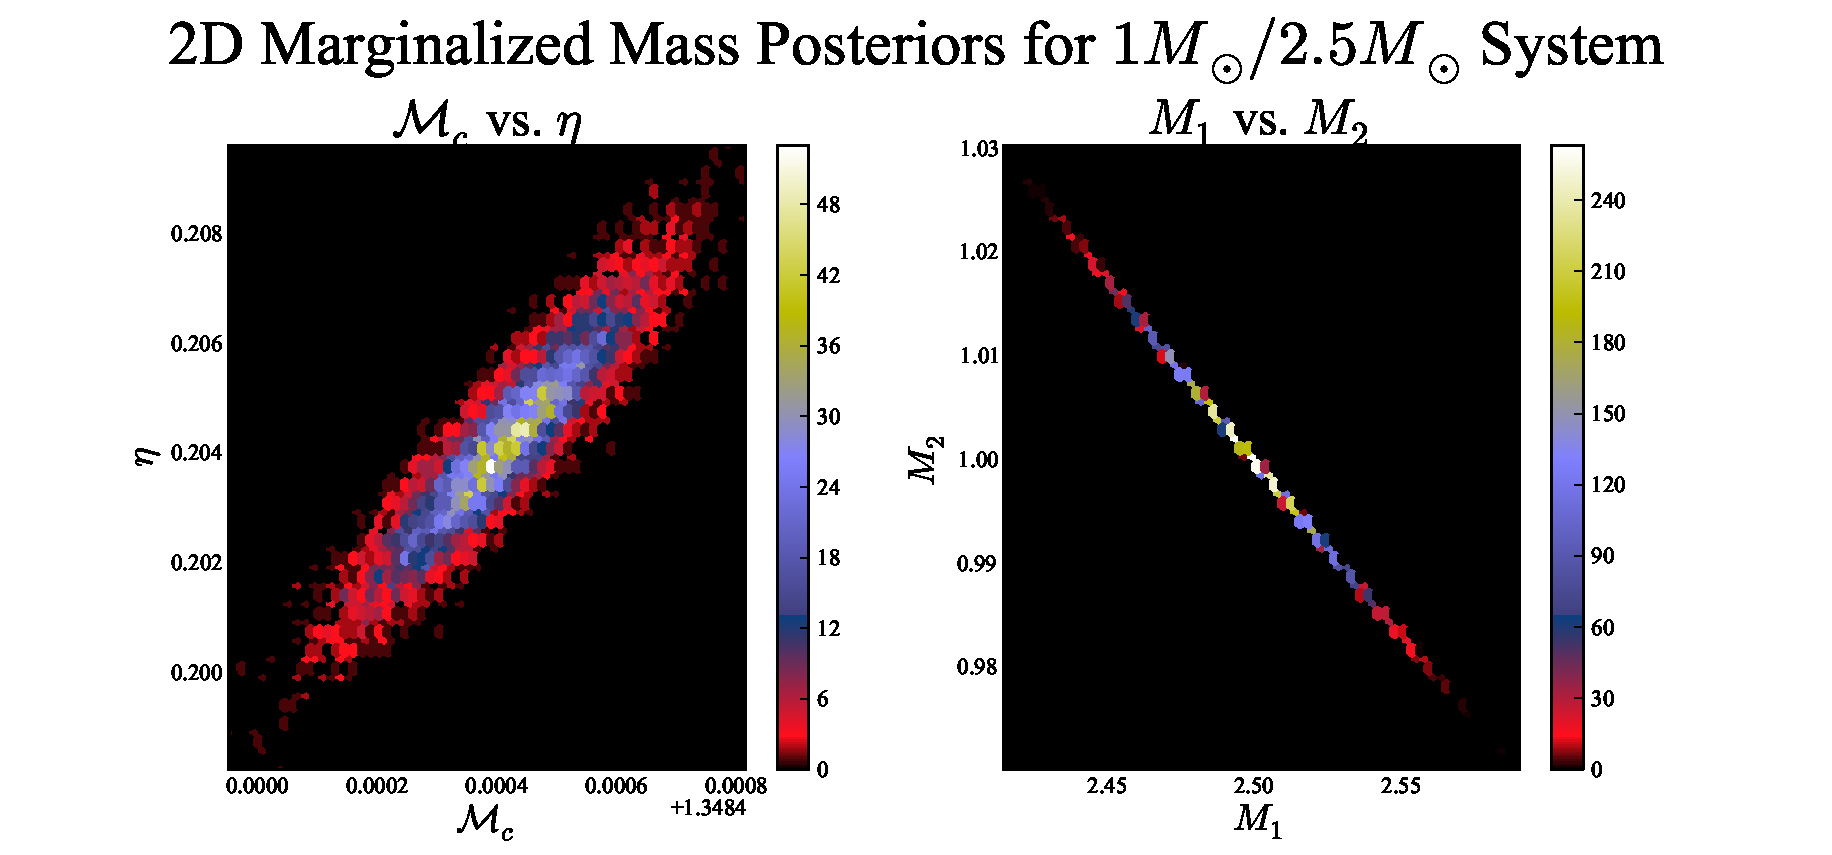
\includegraphics[trim=2cm 0cm 2cm 0cm, clip=true,scale=0.63]{125masses2D.pdf}
 \label{125masses}
 \caption{Similar to figure \ref{1414masses}, for a typical $1M_{\odot}/2.5M_{\odot}$ system.  The unequal mass ratio displaces the posterior PDFs from the $\eta \leq 0.25$ present in the equal mass case, yielding a Gaussian PDF in both the $\mathcal{M}_c$-$\eta$ and $M_1$-$M_2$ spaces.}
\end{figure*}

\begin{figure*}[h!]
  \centering
 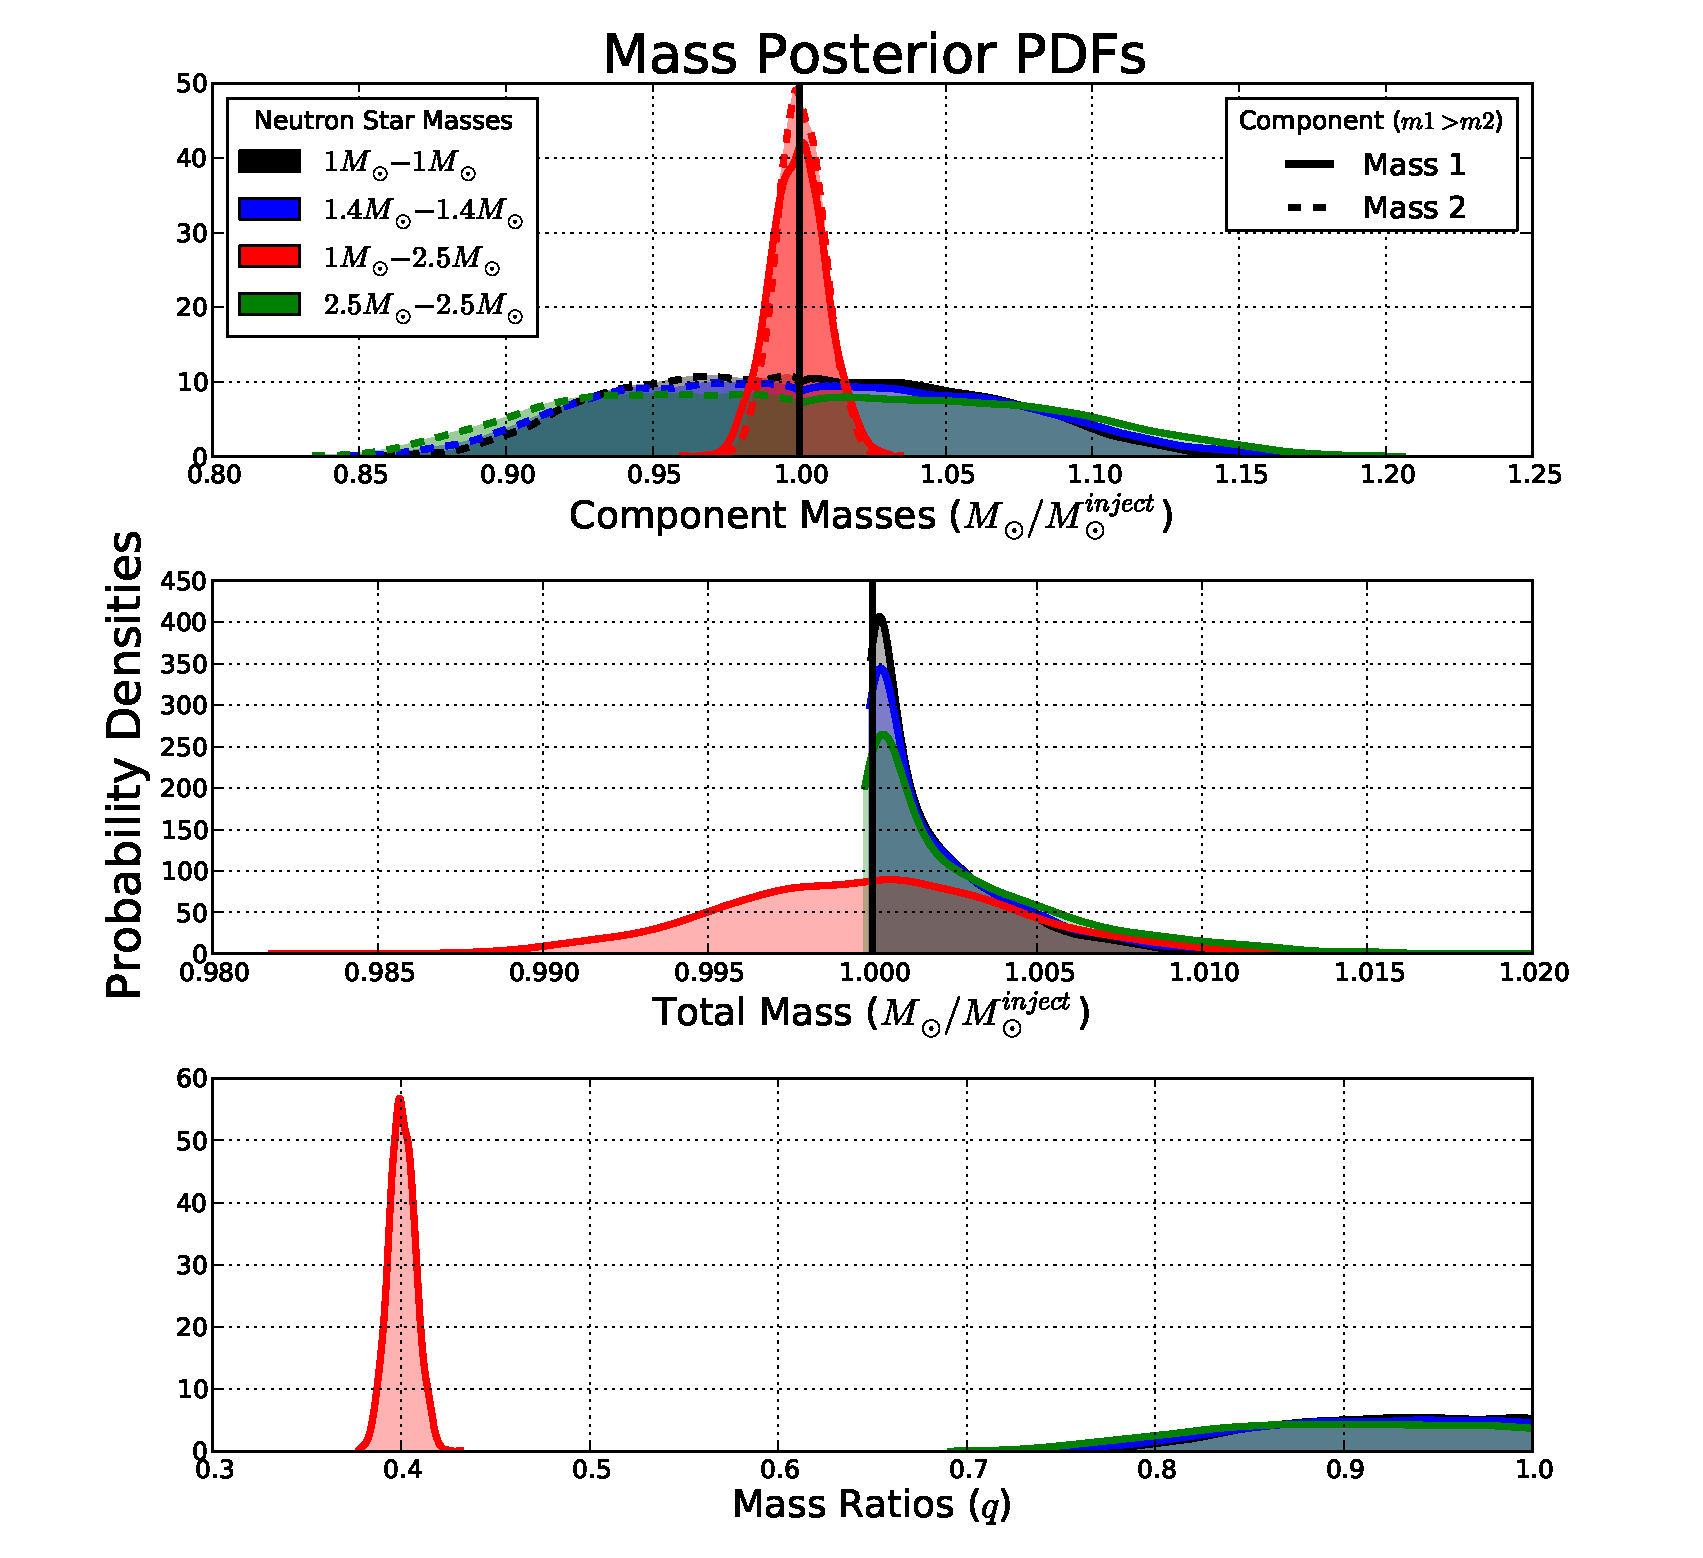
\includegraphics[trim=2cm 0cm 2cm 0cm, clip=true,scale=0.67]{newMasses.pdf}
 \label{masses}
 \caption{Typical 2D mass PDFs for the }
\end{figure*}

%\begin{figure*}[h]
%\begin{center}$
%\begin{array}{cc} 
%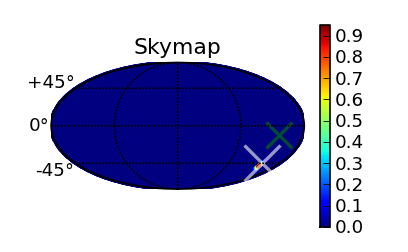
\includegraphics[width=3.2in]{skyPos/2.png} &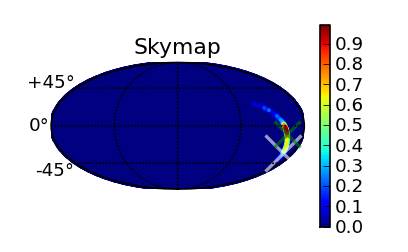
\includegraphics[width=3.2in]{skyPos/4.png}  \\
%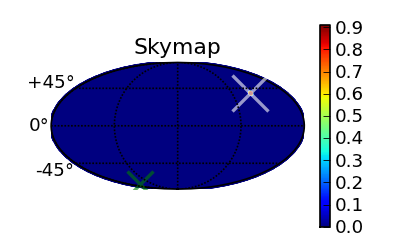
\includegraphics[width=3.2in]{skyPos/5.png} & 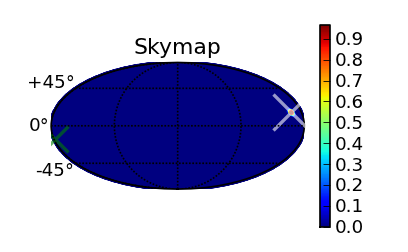
\includegraphics[width=3.2in]{skyPos/7.png} 
%\end{array}$
%\end{center}
%\caption{Example SkyPlots}
%\end{figure*}


\begin{figure*}[tp!]
  \centering
 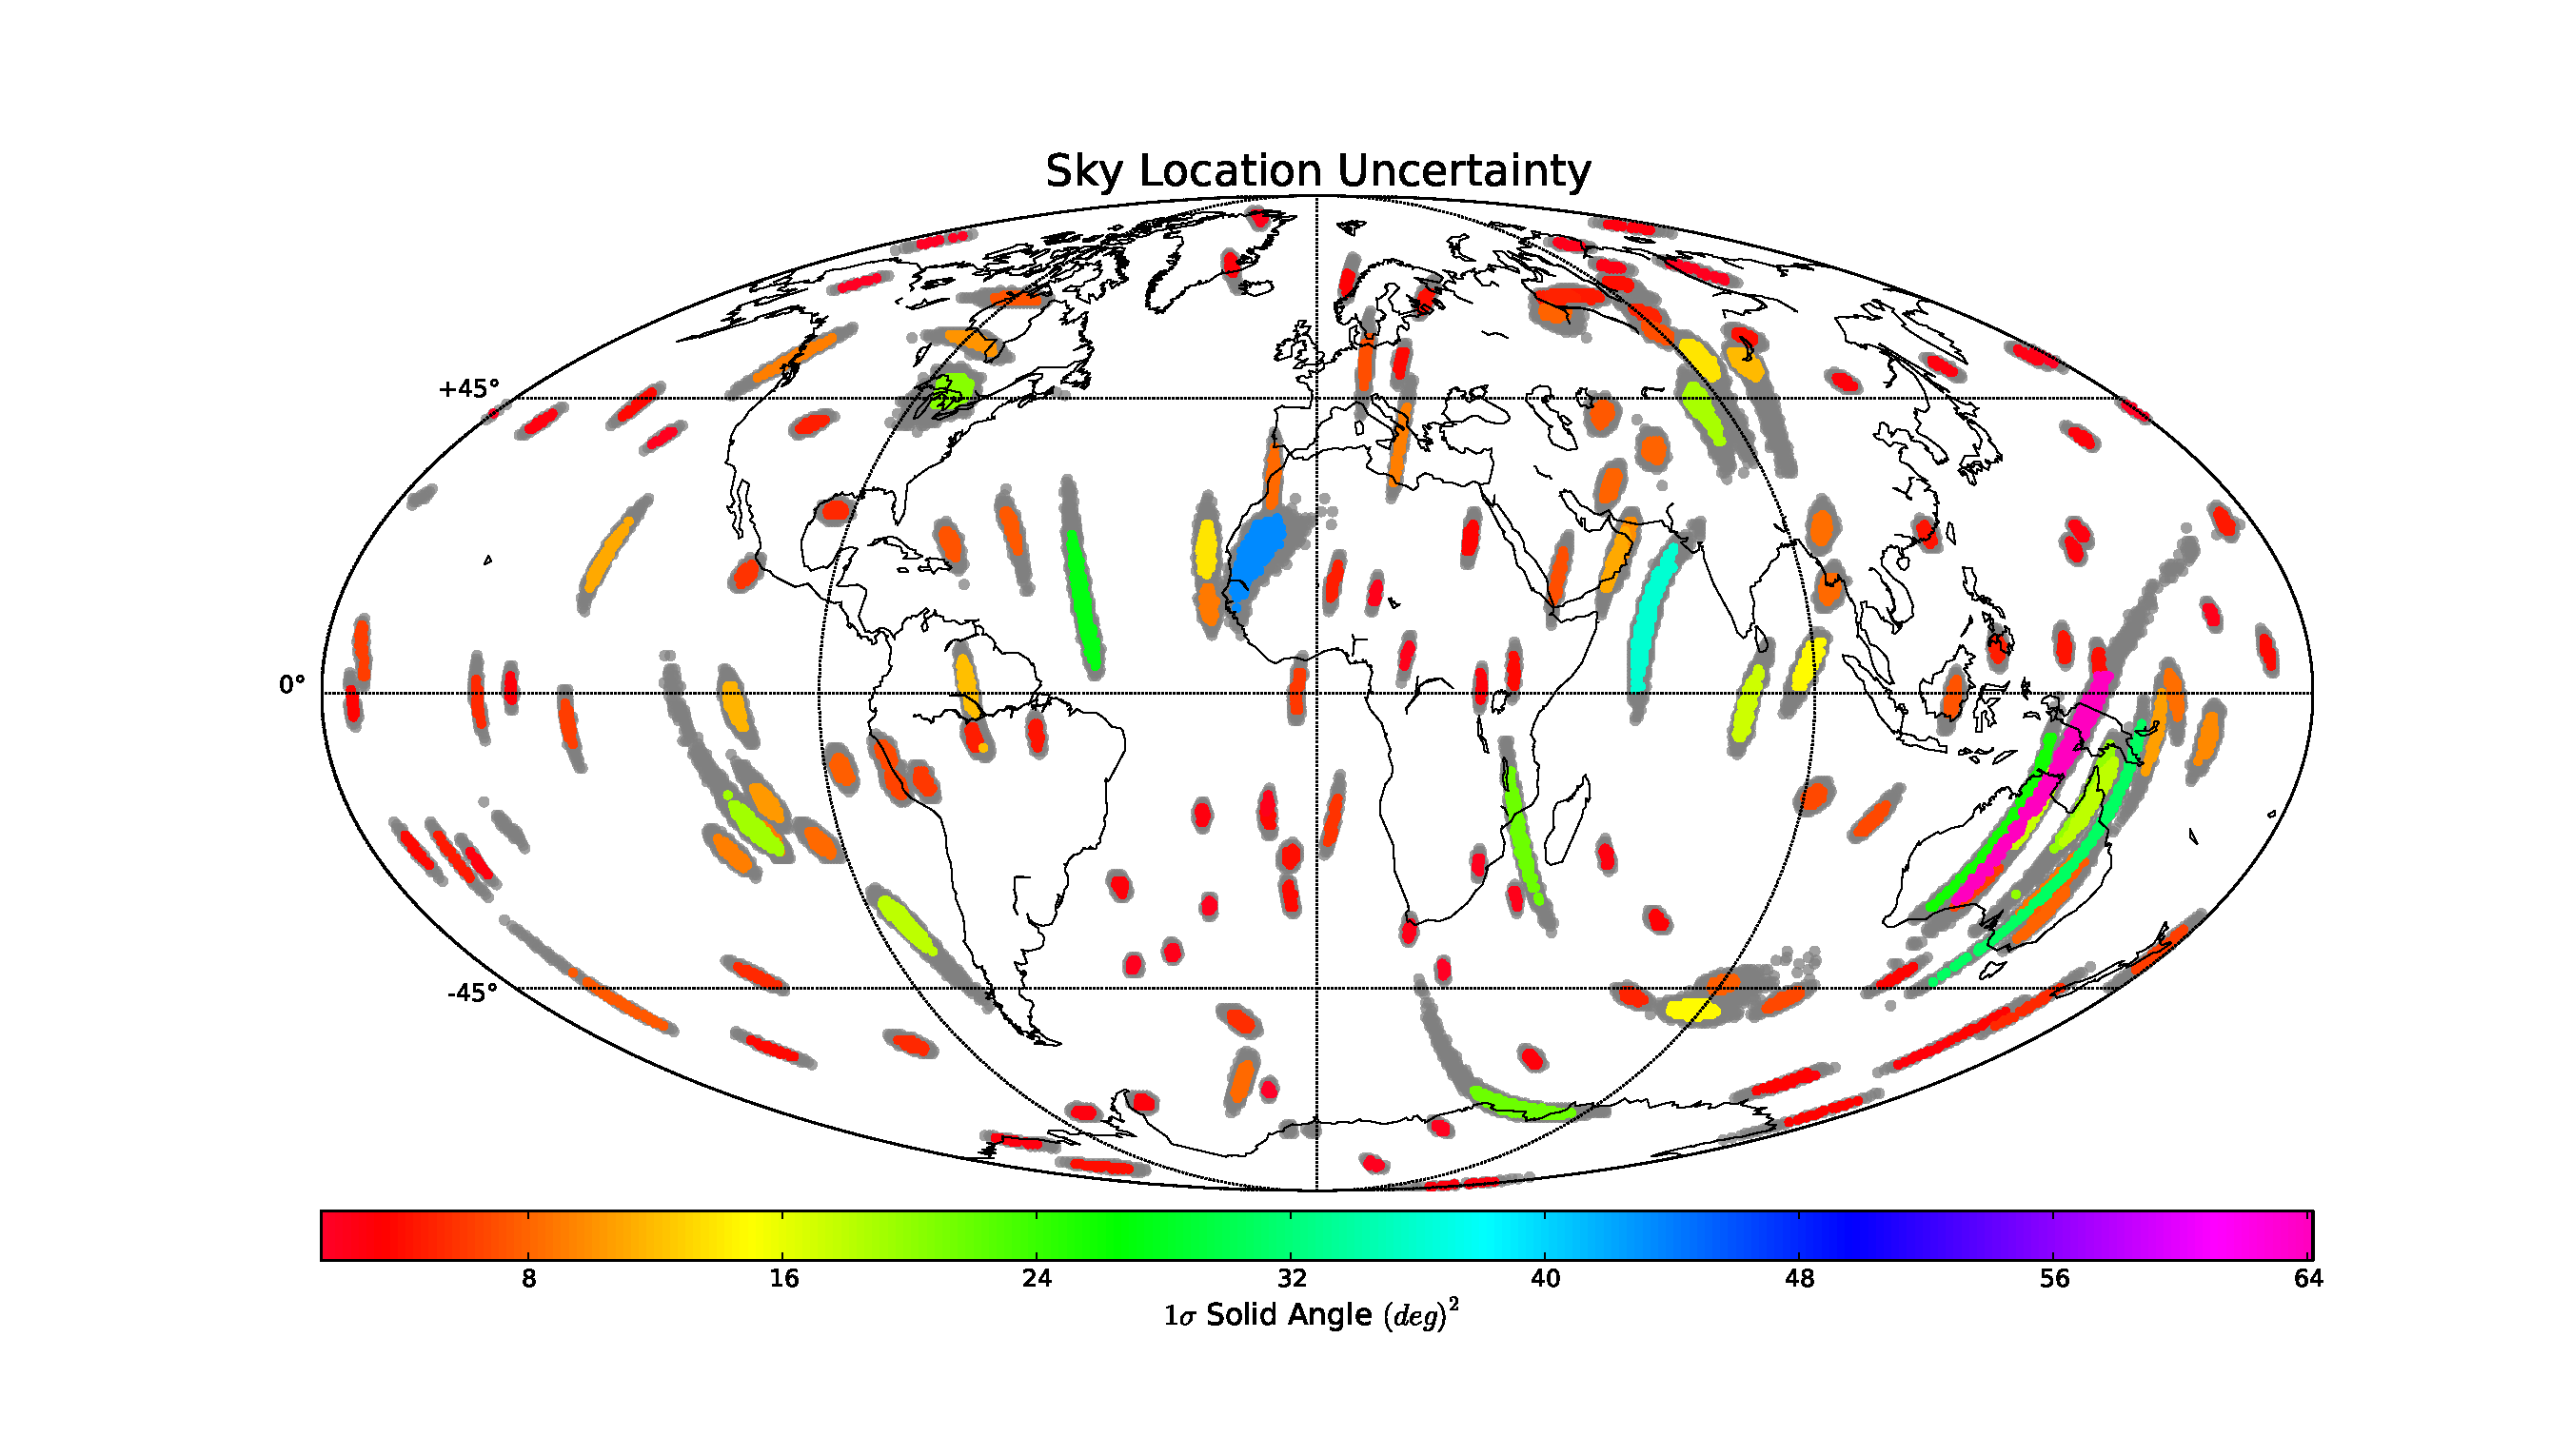
\includegraphics[angle=0,scale=0.49, trim=5cm 0cm 3cm 0cm]{skyLoc.pdf}
 \caption{The uncertainty on the sky of the 160 BNS systems.  Each region represents a single injection, with the colored central region representing the 65\% \carl{[CHECK THAT]} uncertainty region on the sphere, and the gray region representing the 90\% uncertainty region.  The color scheme indicates the total solid angle size of the 65\% region.  Note the similar shape of the uncertainty regions at particular points; this is due to the specific realization of our network pattern sensitivity.}
 \label{2525SkyLoc}
\end{figure*}

   
\begin{figure*}[h!]
  \centering
 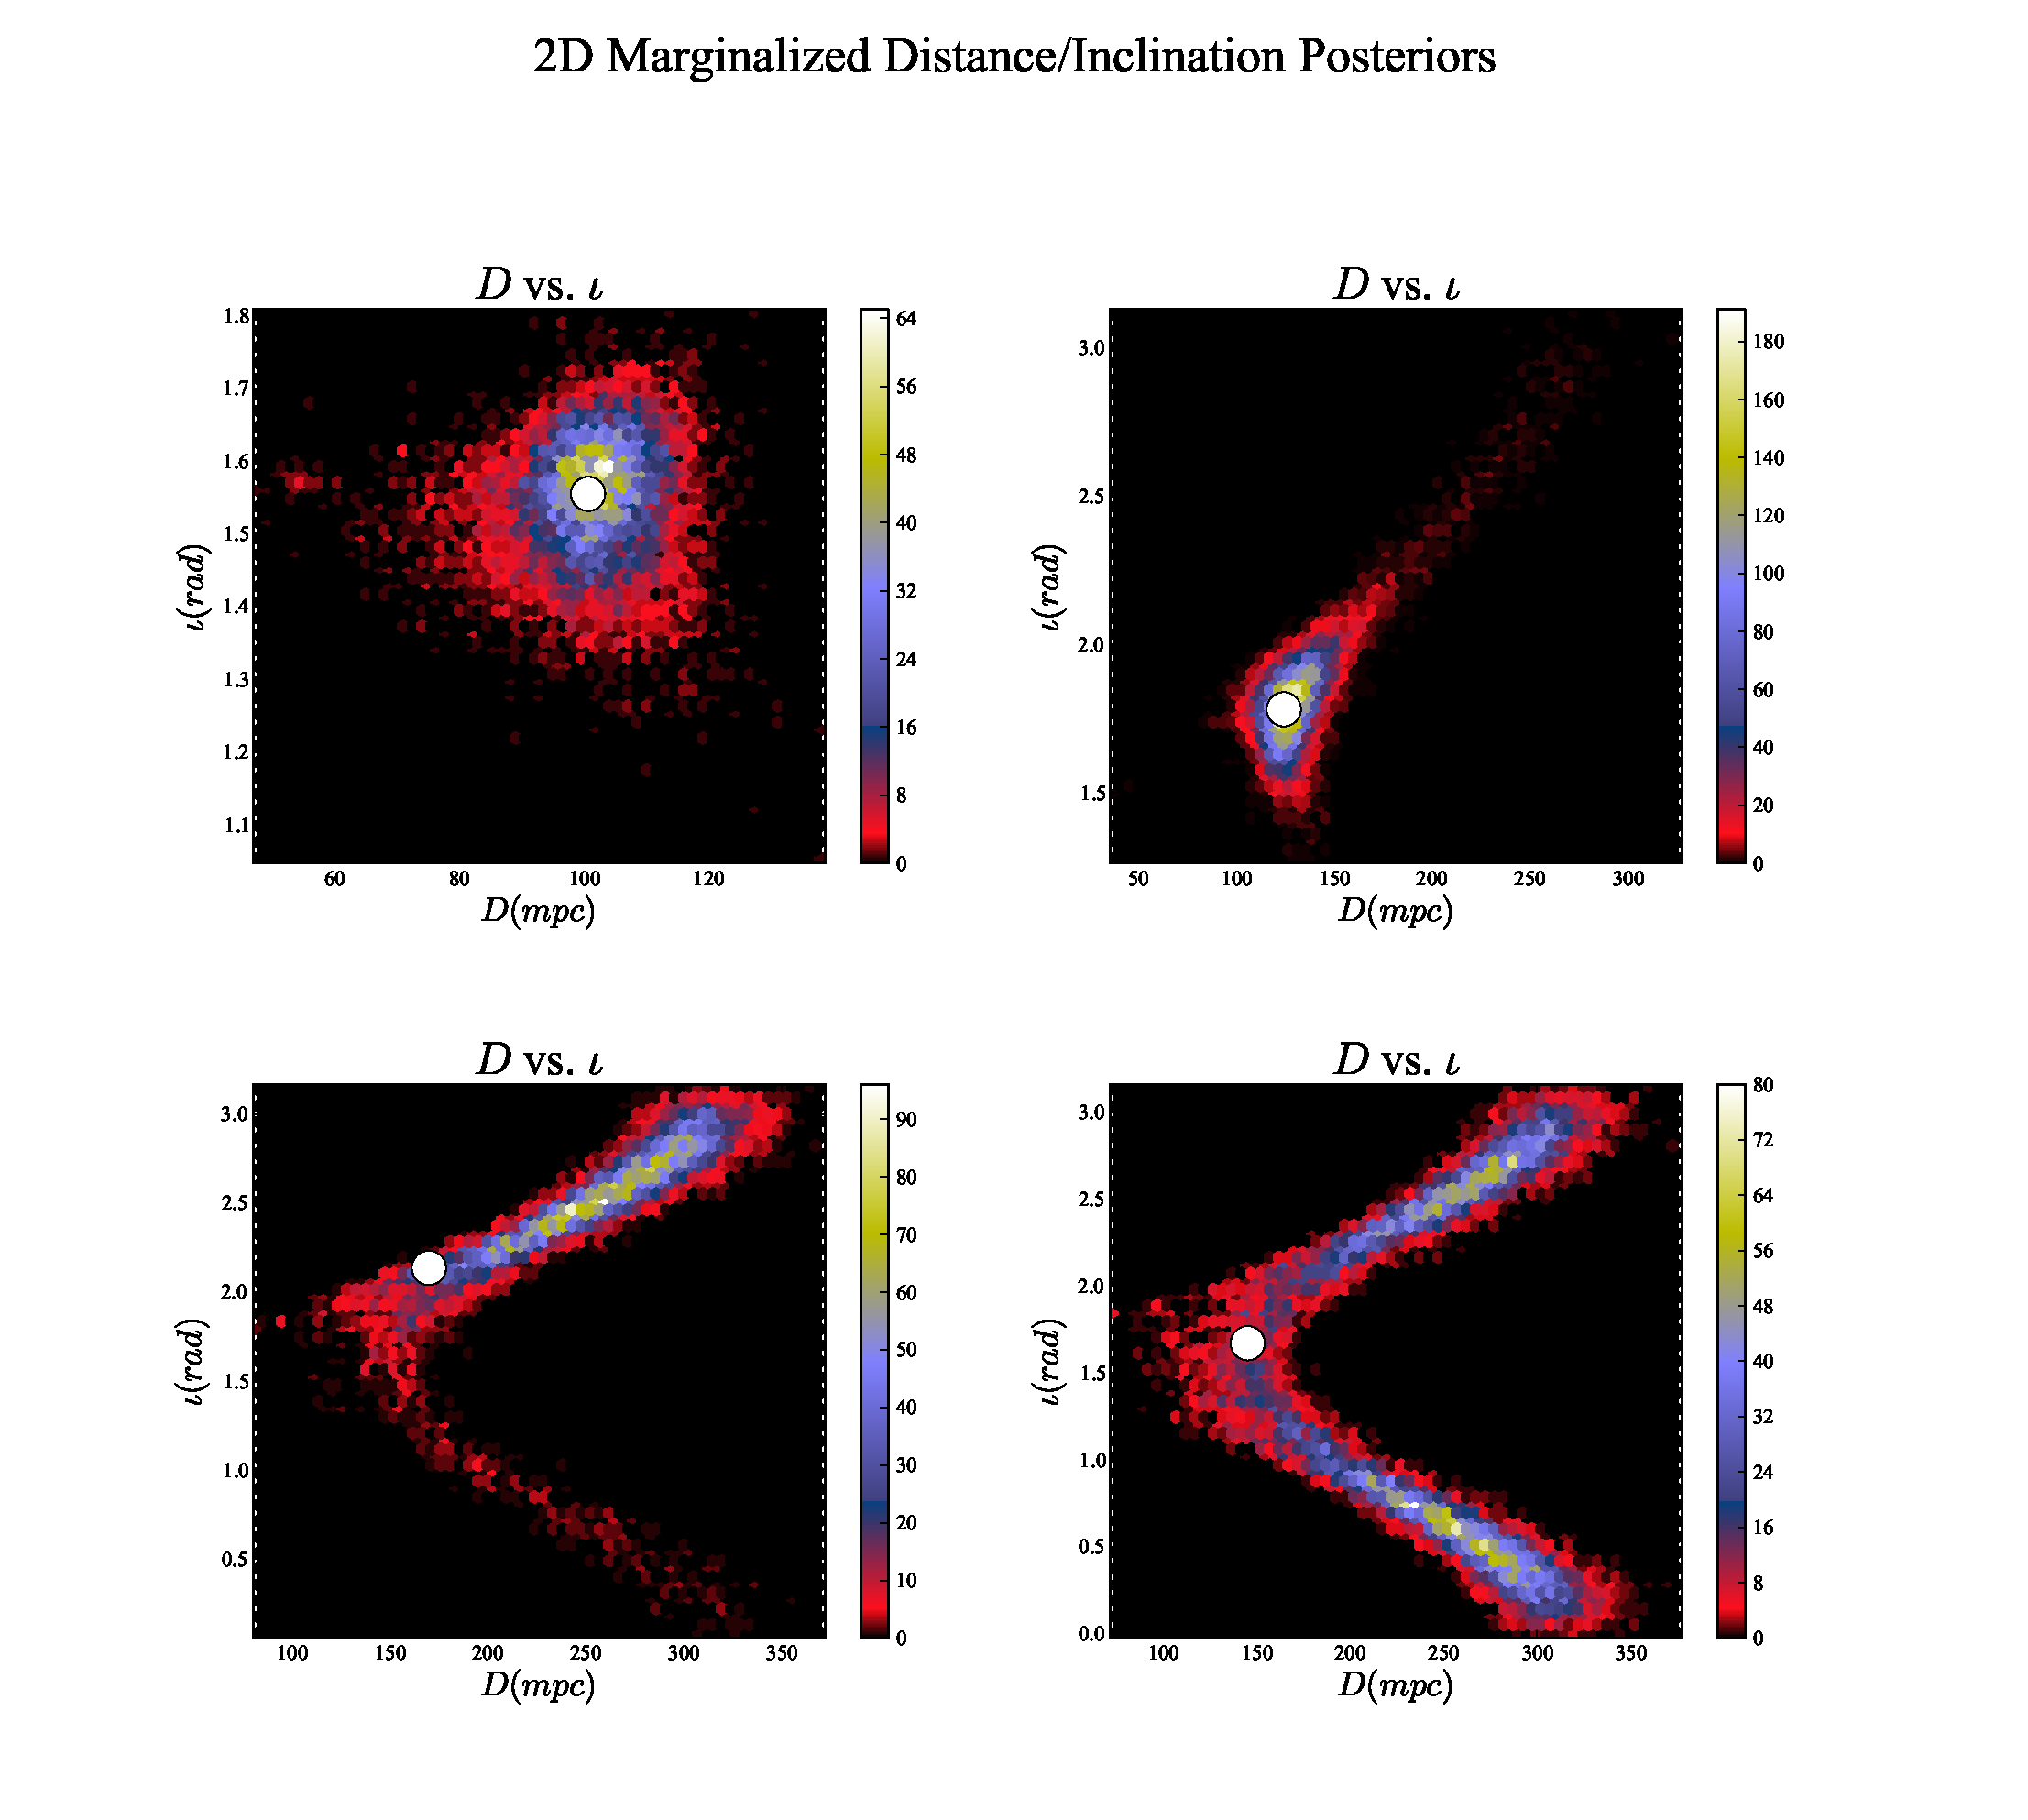
\includegraphics[trim=2cm 0cm 2cm 0cm, clip=true,scale=0.575]{distIota2D.pdf}
 \label{masses}
 \caption{Typical 2D mass PDFs for the }
\end{figure*}


\begin{table*}[t!]
\caption{}
\begin{tabular}{lcccccccccccc}


\hline\hline
System & \vline &  $\Delta \mathcal{M}_c / \mathcal{M}_c$ & \vline & $\Delta \eta$ & \vline & $\Delta M_1/ M_1$ & \vline & $\Delta M_2 / M_2$ & \vline & $\Delta \phi_c$ & \vline &  $\Delta t_c$ (ms)\\
\hline\hline
$1M_{\odot}-1M_{\odot}$ & \vline & & \vline & & \vline & & \vline & & \vline & & \vline &\\
\hline
$1.4M_{\odot}-1.4M_{\odot}$ & \vline & & \vline & & \vline & & \vline & & \vline & & \vline &\\
\hline
$1M_{\odot}-2.5M_{\odot}$ & \vline & & \vline & & \vline & & \vline & & \vline & & \vline &\\
\hline
$2.5M_{\odot}-2.5M_{\odot}$ & \vline & $1.29 \times 10^{-4}$ & \vline & $1.34 \times 10^{-3}$ & \vline & $ 4.01 \times 10^{-2}$ & \vline & $3.65\times 10^{-2}$ & \vline & 1.807 & \vline & 0.418 \\
\hline\hline

\end{tabular}
\label{biasedUnbiasedChirpMassErrors}
\end{table*}


\section{Results}
\label{resultsSection} 

Of the 9 parameters in the domain of the waveform, only 6 are particularly physically interesting: the masses of the two binaries, $M_1$ and $M_2$, the inclination of the binary with respect to the observer, $\iota$, the angular position on the sky, $\alpha$ and $\delta$, and the distance of the source, $D$.

\subsection{Mass Parameters}

Of the 9 variables in our parameter space \eqref{parameterspace}, the two of immediate physical interest are the two parameters, $\mathcal{M}_c$ and $\eta$, or correspondingly the direct masses of the two companions, $M_1$ and $M_2$.    As stated in section \ref{BNSsection}, the ability of Advanced LIGO/VIRGO to construct a population of BNS masses will be critical to the science potential of gravitational-wave astronomy.  

We find that there is virtually no difference between the mass PDFs of our different injected signals within each mass bin.  At first, this may seem disconcerting; however, it is to be expected.  Recall that of the BNS signals were injected with a network SNR of $\rho = 20$ into a zero-noise detector realization.  Furthermore, note that the mass parameters are the only two which directly effect the phase of the TaylorF2 waveform \eqref{phase}.  Therefore, as long as the injected mass parameters are identical within each mass system (they are), and as long as the injected SNR is identical (it is), the amount of recoverable information in each mass parameter should be \emph{almost} identical, and for a sufficiently converged MCMC chain, the recovered posterior PDF should be \emph{almost} identical.  

The ``almost'' in the previous sentence is to draw attention to one critical, neglected fact: while the mass parameters are independent of the injected signals position with respect to the detector network, the other parameters are certainly not.  Obviously many of the other parameters (i.e. sky location, polarization, distance, inclination, and time-of-arrival) all depend on the orientation of the binary inspiral with respect to each of the individual detector locations.  Since our 9-dimensional parameter space can be highly correlated, it is entirely reasonable to assume that cross-correlations between the extrinsic parameters and the mass parameters will cause variation in the recovery of the individual injection PDFs.  

In practice, it was found that the cross-correlations between the extrinsic parameters and signal time-of-arrival were several orders of magnitude \carl{[QUANTIFY THIS]} below the uncertainties in $\mathcal{M}_c$ and $\eta$.  It should be noted that, in practice, this will \emph{not} be the case: in reality, the noise power-spectral density of each detector varies as a function of time, including both natural variations in sensitivity and detector glitches \carl{[CITE SOMETHING]}.  In such a case, the base sensitivity of a gravitational-wave detector to even the easiest to recover parameters will vary as a function of position and time.  What we report here can thus be considered an idealized, ``glitch-free'' world in which each detector has an identical noise realization at all times.  In Section \ref{NoisySubSection}, we provide each detector with a random, but not identical, noise model based on the Advanced LIGO PSD, thus giving an insight into this time-dependent variation \carl{[PLEASE TELL ME THAT'S WHAT LALINFERENCE DOES...]} (while still ignoring instrumentation glitches).

In Figures \ref{1414masses} and \ref{125masses}, we show the marginalized 2D posterior PDFs of our mass parameters a prototypical equal mass and unequal mass binaries.  We include the PDF in both the $\mathcal{M}_c$-$\eta$ space (relevant for the waveform), and the more physically interesting component mass space ($M_1$-$M_2$).  Although only the $1.4M_{\odot}/1.4M_{\odot}$ system is included in Figure \ref{1414masses}, the PDF is virtually identical to the other equal mass cases, modulo a scaling factor.  Again, this is unsurprising due to the identical SNR of each of the injected signals.   

\subsection{Sky Localization}

\subsection{Inclination and Distance}

\begin{enumerate}
\item Inclination for GRB folks
\item Distance for population studies
\item degeneracy between the two
\end{enumerate}

\subsection{Varied Noise Realizations}
\label{NoisySubSection}
\subsection{Testing MCMC Convergence}

\carl{include a paragraph on our standard convergence checks}.  However, there is an additional check we can consider: the standard matched filtering searches employed by the LIGO/VIRGO collaboration assume that a detection will occur when one of the template waveforms matches the detector data with a signal overlap of 97\% or better \carl{cite something}.  That is, for a template waveform $h^{t}(f)$ and detector output $s(f)$, an overlap of

\begin{equation}
\left< s | h^{t}\right> \geq 97\%
\nonumber
\end{equation}

\noindent  yields a detection.  This requirement provides us with a convenient test for the effectiveness of our parameter estimation.  First, we note that maximizing our likelihood function, \eqref{likelihood}, is identical to maximizing the SNR \eqref{formalSNR} of our template waveform in a given stretch of data.  Therefore, the better the match between the template waveform and the data, the higher the SNR.  Since we assume, quite tautologically, that our parameter estimation code should estimate parameters at least as well as a matched filtering approach, we would be immediately suspicious of any MCMC run whose maximum-likelihood waveform had an SNR below that of our pipeline trigger.   In that case, we would perform the MCMC with a much longer runtime, until the maximum likelihood of our posterior distribution had an SNR at least as high as the detection.

For the purposes of our present study, we reproduce this information as follows: since we know the true SNR of the signal we are simulating, we assume that the ``trigger'' SNR returned by our detection pipeline is 97\% of the true SNR.  We then assume any posterior distribution whose maximum likelihood satisfies

\begin{equation}
\text{Maximum Likelihood} \leq 0.97 \times \left(\frac{\rho_{inj}^2}{2}\right) 
\nonumber
\end{equation}

\noindent has not converged.  As one would expect, the lower-mass, longer waveform systems require longer to converge.  With our original runtime of one week over 8 processors, we found that seven of our $1M_{\odot}/1M_{\odot}$ systems had not converged, while all but one system for our $1.4M_{\odot}/1.4M_{\odot}$ and $1M_{\odot}/2.5M_{\odot}$ systems had converged.  All of the $2.5M_{\odot}/2.5M_{\odot}$ systems converged within the week.  

We performed a second run for each of the non-converged systems

\bibliographystyle{apj}
\bibliography{paper}{}

\end{document}
